\section{Hardware}

\begin{figure}[h]
	\centering
	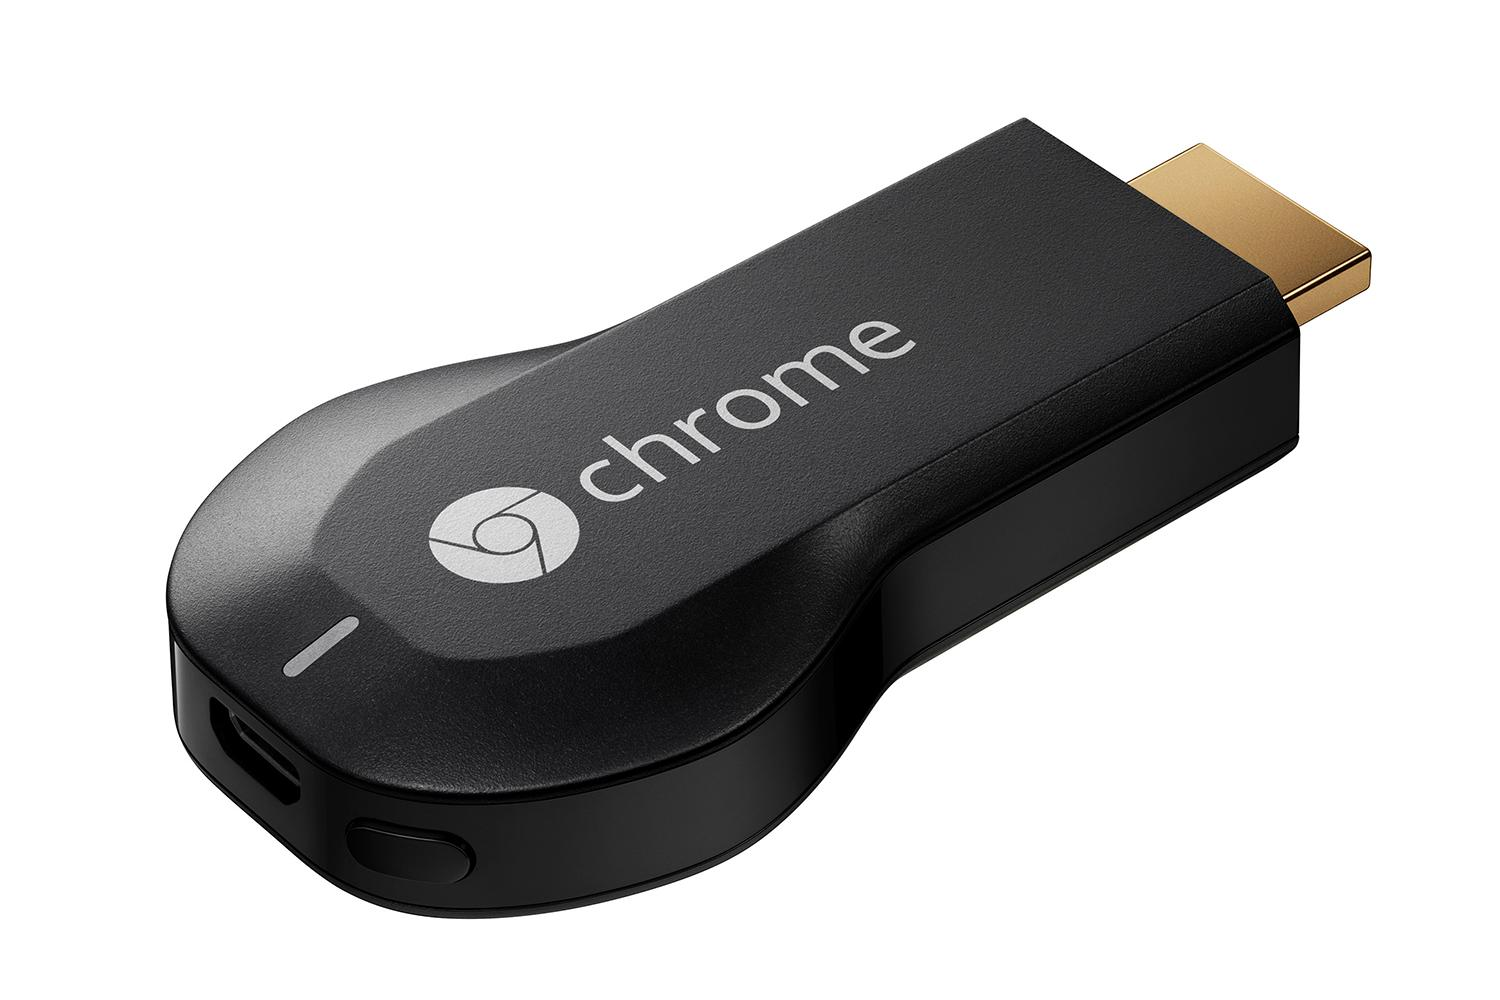
\includegraphics[width=0.49\textwidth]{./Imagenes/chromecast1gen.jpg}
	\caption{Chromecast de primera generación}\label{fig:1gen}
\end{figure}

El Chromecast de primera generación incluye un decodificador de VP8 y H.264 para formatos de compresión de vídeo, 512 MB de Micron DDR3L RAM y 2 GB o 4 GB de memoria flash según la fuente (Google no ha publicado las especificaciones del dispositvo).
Se conoce que tiene un chip a 700 MHz single core.
Tiene una salida HDMI, una entrada micro USB para la alimentación, un LED que indica el estado del dispositivo y un botón para el reseteo.
Sus estándares de conexión son Wi-Fi 802.11 b/g/n (solo 802.11n a 2,4 GHz).

\

El de segunda generación tiene 512 MB de Samsung DDR3L RAM y 256 MB de memoria flash.
El dispositivo tiene un cable flexible en cuyo extremo se encuentra la salida HDMI, usa un procesador dual core ARM Cortex-A7 con 1.3 GHz de frecuencia y tiene tres antenas adaptativas para mejorar la conexión con el router.
Sus estándares de conexión son 802.11 b/g/n/ac Wi-Fi (2,4 GHz/5 GHz).

\begin{figure}[h]
	\centering
	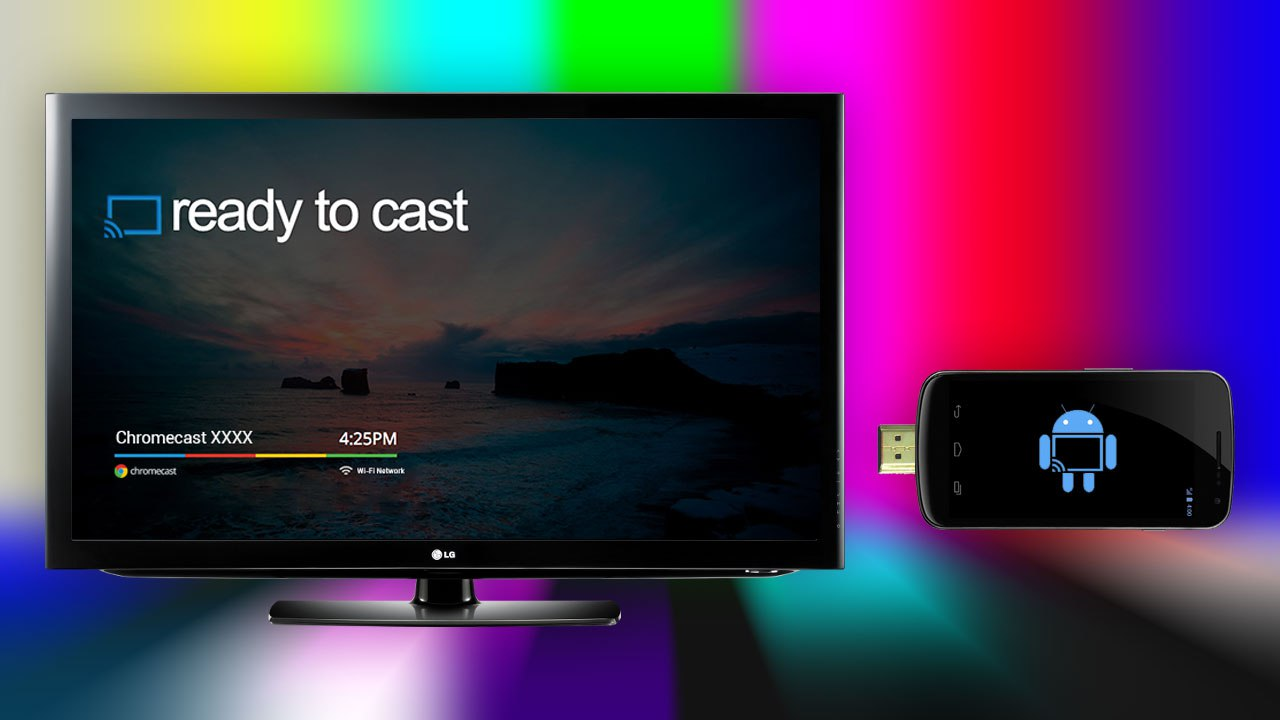
\includegraphics[width=0.49\textwidth]{./Imagenes/chromecast.jpg}
	\caption{Chromecast de segunda generación}\label{fig:2gen}
\end{figure}

El Chromecast Audio es externamente igual que el de segunda generación, pero tiene una salida Jack de 3,5\" en lugar del HDMI y un chip de procesamiento de audio.

\begin{figure}[h]
	\centering
	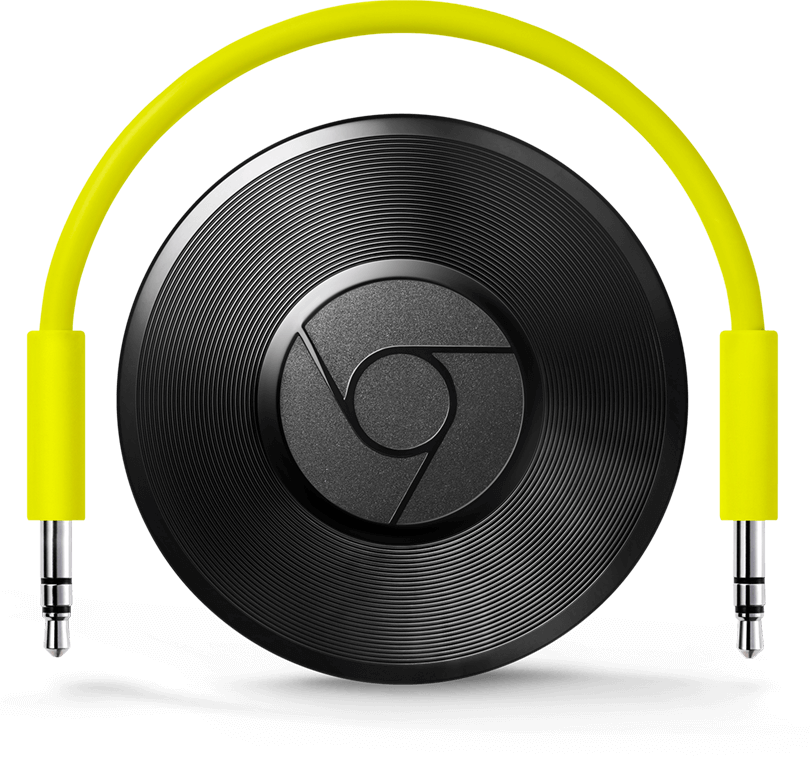
\includegraphics[width=0.38\textwidth]{./Imagenes/chromecastaudio.png}
	\caption{Chromecast Audio}\label{fig:audio}
\end{figure}

Acerca del hardware del Chromecast Ultra se conoce poco de manera oficial.
La mayor diferencia es, aparte de la mayor potencia de procesamiento nesearia para reproducir vídeo 4K, que incluye una entrada Ethernet en el adaptador de corriente para conectarlo a Internet como alternativa al Wi-Fi.

\begin{figure}[h]
	\centering
	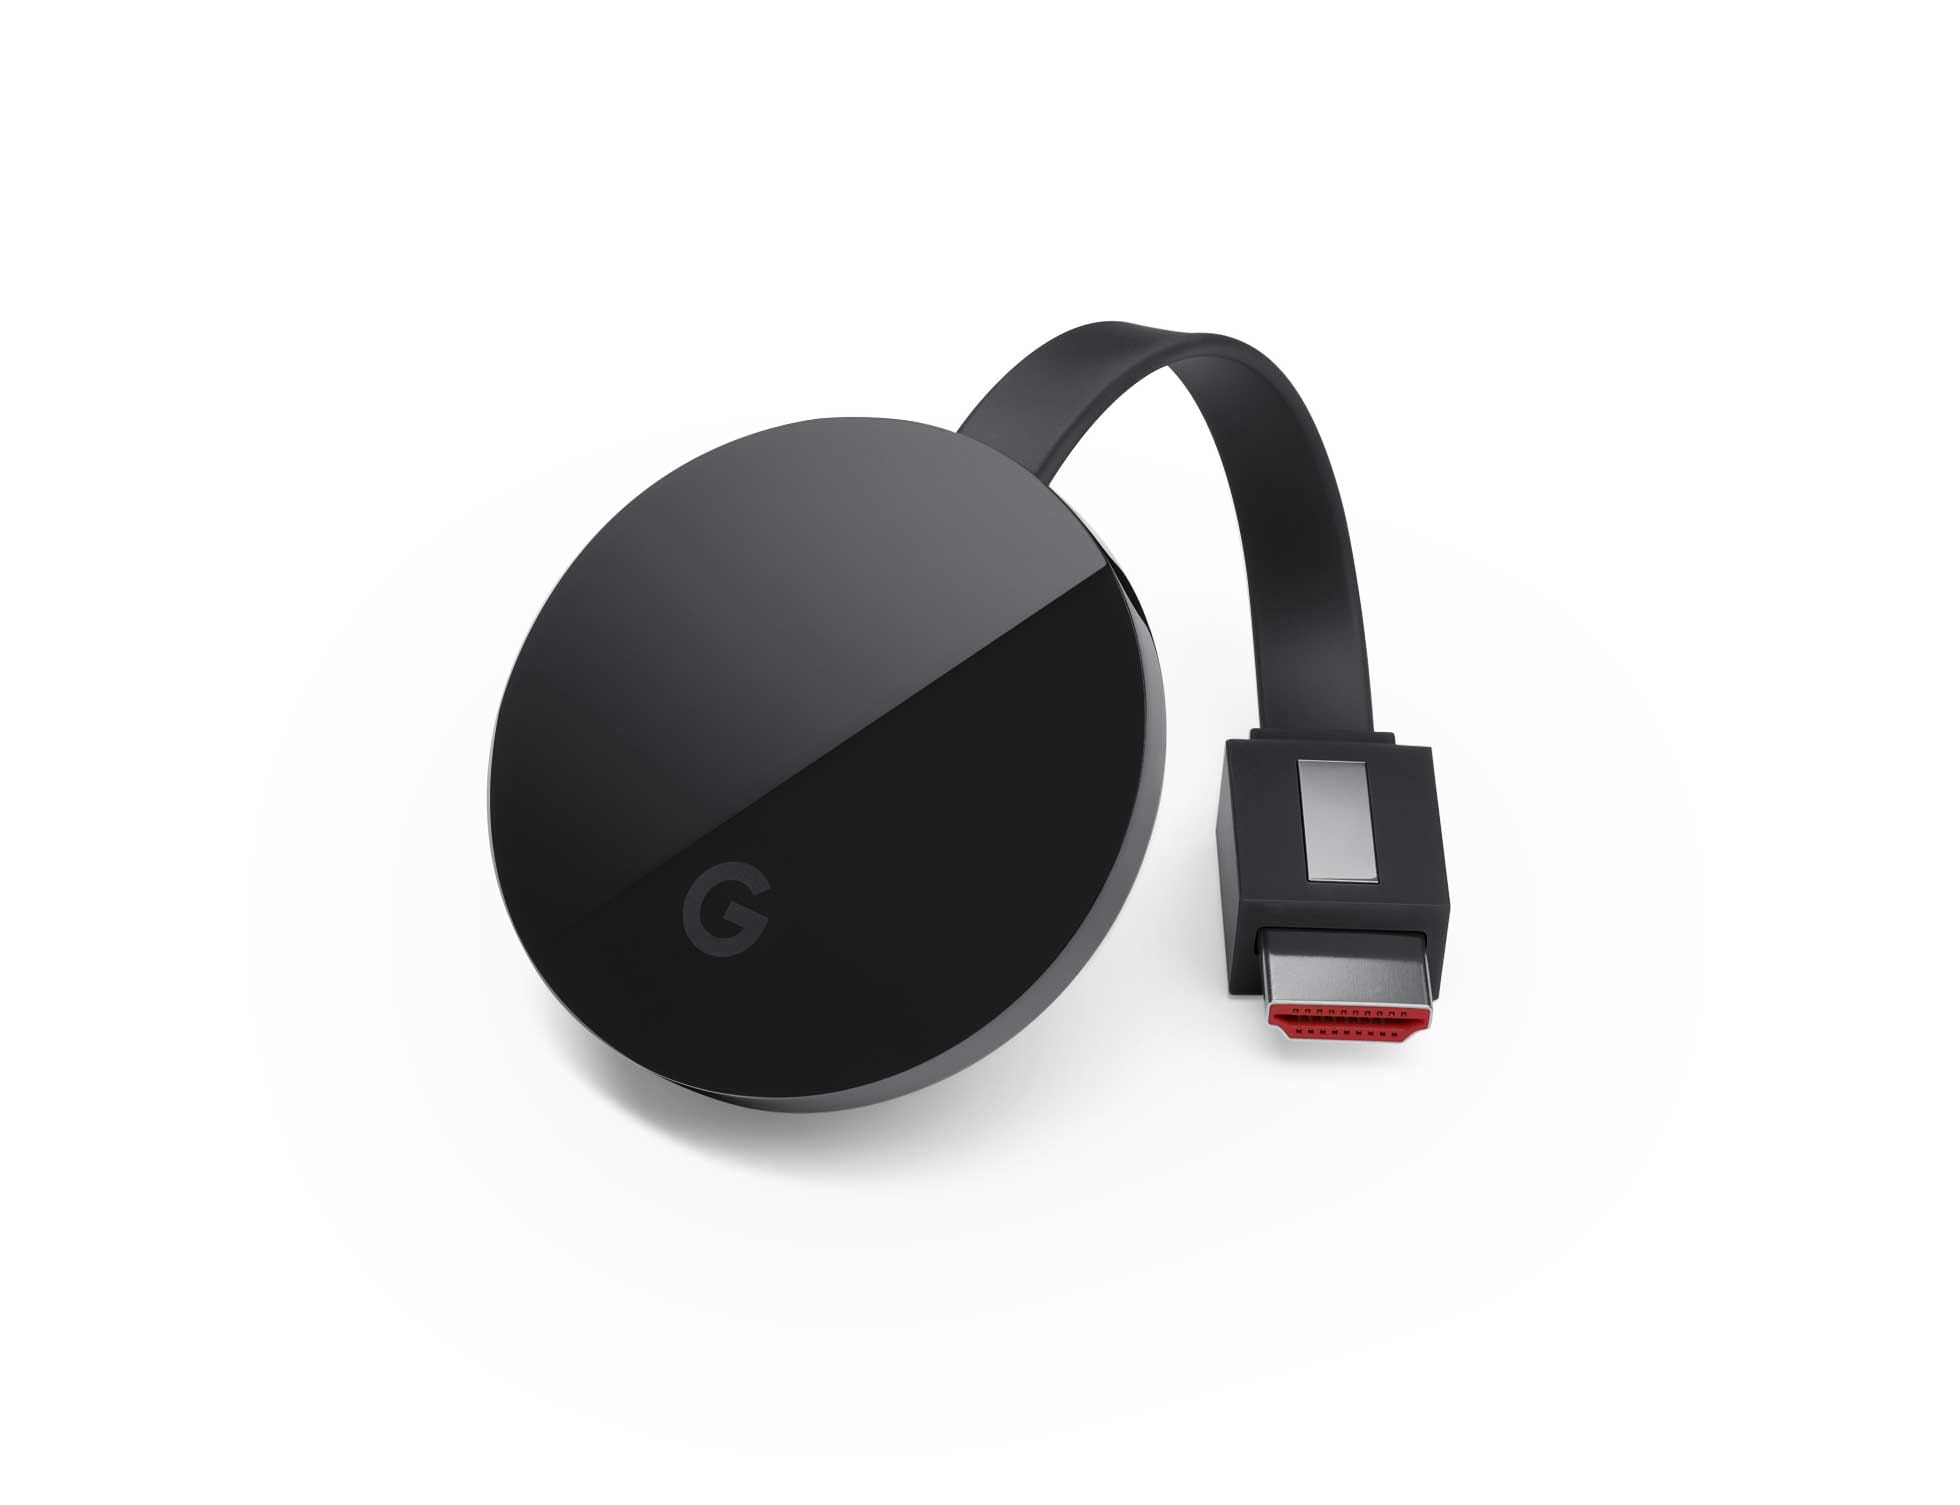
\includegraphics[width=0.49\textwidth]{./Imagenes/chromecast-ultra.jpg}
	\caption{Chromecast Ultra}\label{fig:ultra}
\end{figure}
